\documentclass[a4paper]{article} % For LaTeX2e
\usepackage[T1]{fontenc} % add special characters (e.g., umlaute)
\usepackage[utf8]{inputenc} % set utf-8 as default input encoding
\usepackage{ISMIRlbd, cite, times, amsmath, url}
\usepackage{hyperref}
\usepackage{url}
\usepackage{float}
\usepackage{graphicx}
\usepackage{booktabs}
\usepackage{color}
\usepackage{amsfonts}

\title{\MakeLowercase{flow}EQ: A smarter equalizer plugin using a disentangled variational autoencoder}


% Note: Please do NOT use \thanks or a \footnote in any of the author markup

% Single address
% To use with only one author or several with the same address
% ---------------
%\oneauthor
% {Names should be omitted for double-blind reviewing}
% {Affiliations should be omitted for double-blind reviewing}

% Two addresses
% --------------
%\twoauthors
%  {First autho} {School \\ Department}
%  {Second author} {Company \\ Address}

%% To make customize author list in Creative Common license, uncomment and customize the next line
\def\authorname{Christian Steinmetz, Xavier Serra}

\oneauthor
  {Christian Steinmetz  Xavier Serra} {Music Technology Group, Universitat Pompeu Fabra, Barcelona (Spain) \\ {\tt christian.steinmetz@upf.edu}}

\newcommand{\fix}{\marginpar{FIX}}
\newcommand{\new}{\marginpar{NEW}}

%\iclrfinalcopy % Uncomment for camera-ready version, but NOT for submission.
\begin{document}


\maketitle

\begin{abstract}

% [ main abstract ]

We present \textbf{flowEQ}, an intelligent interface for a five-band parametric equalizer plugin. \textbf{flowEQ} enables the audio engineer to control the all thirteen parameters of the equalizer using either one, two, or three knobs (a user-controllable parameter). This is achieved by learning low dimensional mappings from 1, 2, and 3 dimensional latent spaces to the thirteen dimensional parameter space of the equalizer with the use of a variational autoencoder. Additionally, different levels of latent space disentanglement are investigated providing the user with the ability to adjust the latent representations directly within the plugin. By traversing the latent spaces of the trained models, the user can quickly search through relevant configurations of the equalizer. This methodology promotes using one’s ears to determine the proper EQ settings and enables both novice and experienced audio engineers to more efficiently apply timbral processing in the post-production process.

% [ plugin screenshot ]

\begin{figure}[H]
  \centerline{
  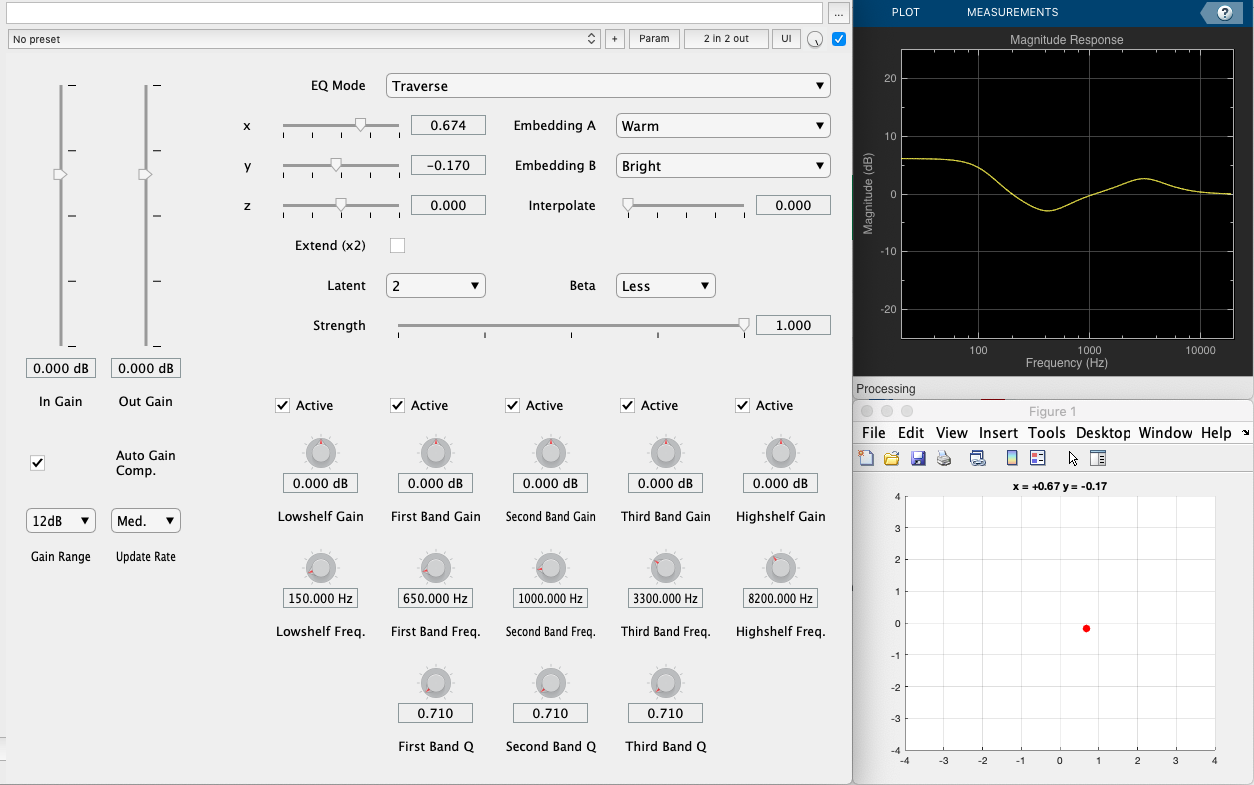
\includegraphics[width=0.6\columnwidth]{../../img/full_visual.png}}
  \caption{VST plugin running in REAPER with real-time MATLAB visualization tool.}
  \label{fig:plugin}
 \end{figure}

% [ introduction ]

The parametric equalizer is the de-facto tool used by audio engineers to shape the timbral content of an audio signal. First introduced with analog circuitry in the early 1970s \cite{massenburg}, these processors have evolved with the advent of digital signal processing and are readily available as plugins or standalone outboard processors.  is one of the most powerful forms of the equalizer, since it provides direct control over the gain, center frequency, as well as the bandwidth (known as the Q factor) for each band. Most parametric equalizers feature multiple bands, allowing extensive control over the processor’s transfer function. 

Due to the increased complexity of the parametric equalizer in comparison to other forms of equalizers, such as bass and treble controls or graphic equalizers, additional experience is required on the part of the audio engineer in order to achieve the desired timbral effect. The goal of \textbf{flowEQ} is to provide a simplified interface with embedded information on relevant configurations of the equalizer. 

% [ previous work ]

Previous work has investigated the use of timbral semantics for the intelligent control of different equalizers. In \cite{cartwright_socialeq}, the authors use crowdsourced data to uncover universal, semantic descriptors of timbre with the goal of designing an equalizer that can respond to descriptive language directly. 

The SAFE project plugins \cite{safe2014}, which include a compressor, distortion, reverb, and a parametric equalizer, provide a means to collect semantic user data directly from the normal workflow of audio engineers. The work presented in \cite{stasis_reduce_dimension} is the most similar to \textbf{flowEQ}, and attempts to use data from the SAFE equalizer to build a two dimensional model for controlling the ‘warmth’ and ‘brightness’ of the timbral transformation. Different methods of dimensionality reduction are investigated along with a vanilla autoencoder structure. While these semantic interfaces present potentially promising results in the control of an equalizer, they are inherently limited by the generalization and relative specificity of the semantic descriptors studied. \textbf{flowEQ} both improves and expands upon this work by employing a more modern and powerful model, the variational autoencoder, along with the investigation of variable latent space dimensionality and disentanglement. 

% [ method ]

We use the VAE formulation originally presented in \cite{vae} where we attempt to jointly learn the parameters, $\phi$ and $\theta$, of the probabilistic encoder, $q_\phi(\mathbf{x}|\mathbf{z})$, and the generative model $p_\theta(\mathbf{z}|\mathbf{x})$.

During optimization we minimize the expected negative log-likelihood for the data generated by the decoder, $p_\phi(x_i|z)$, after sampling a latent code from the encoder, $z \sim q_{\theta}(z|x_i)$. 
This acts as a reconstruction loss, incentivising the model to accurately encoder and decode the inputs. An additional regularization term is included, the KL divergence,  incentives the model to the encode inputs similarly to the isotropic multivariate Gaussian, $p_\theta(\mathbf{z}) = \mathcal{N}(\mathbf{z};0,\mathbf{I})$.

Equation \ref{eq:loss} shows the loss function used, with the addition of a hyperparameter $\beta$, known as the disentanglement factor \cite{higgins_betavae}. 


\begin{equation}
  \mathcal{L}(\pmb{\theta},\pmb{\phi},\mathbf{x}^{(i)}) = - \mathbb{E}_{\mathbf{z} \sim q_{\theta}(\mathbf{z}|\mathbf{x}^{(i)})} [ {\log{p_\phi(\mathbf{x}^{(i)} | \mathbf{z})}} ] + \mathbf{\beta} \: D_{KL} (q_\theta(\mathbf{z} | \mathbf{x}^{(i)}) || p_\theta(\mathbf{z})).
  \label{eq:loss}
\end{equation}

% [ implementation ] 

The plugin is implemented with the MATLAB Audio Toolbox \footnote{https://www.mathworks.com/products/audio.html}, which provides an API for compiling MATLAB code directly to VST/AU plugins to be executed in a host, most commonly DAWs. Compiled plugins for macOS and Windows are made available on the project website\footnote{https://flowEQ.ml/}. Three modes of operation are features: Traverse, Semantic, and Manual. 
Traverse mode allows the user to directly sample from the latent space of the selected model. This utilizes either 1, 2, or 3 sliders on the UI based upon the dimensionality of the selected model. In semantic mode the descriptor labels are used to build a linear model in each of the latent space spaces. Pre-computed semantic embeddings are provided and the user has the ability to interpolate between two different selected embeddings within the latent space. Finally, Manual mode allows the user to directly control each of the parameters in the equalizer.  

% [ conclusion ]

\textbf{flowEQ} provides an intelligent modality for interfacing with the parameter space of the five band parametric equalizer. The user additionally has control over the latent space representations used during the transformation, with direct control over the dimensionality and disentanglement present.


%\begin{table}[h]
%  \label{sample-table}
%  \begin{center}
%  \begin{tabular}{l|cccccccccccc}
%  \toprule
%  \textbf{Model} & \textbf{1} & \textbf{2}  & \textbf{3}  & \textbf{4}  & \textbf{5}  & \textbf{6}  & \textbf{7}  & \textbf{8}  & \textbf{9}  & \textbf{10}  & \textbf{11}  & \textbf{12} \\
%  \midrule
%  Latent    &      1D &   1D   &   1D    & 1D & 2D  & 2D & 2D & 2D & 3D & 3D & 3D & 3D \\
%  Beta  & 0.000   &  0.0001    & 0.01 & 0.02 & 0.000 & 0.0001 & 0.01 & 0.02 & 0.000 & 0.0001 & 0.01 & 0.02\\
%  \bottomrule
%  \end{tabular}
%  \caption{Sample table title}
%  \label{tab:example}
%  \end{center}
%\end{table}

% [ conclusion ]


\end{abstract}

%\section{Final instructions}
%Do not change any aspects of the formatting parameters in the style files.
%In particular, do not modify the width or length of the rectangle the text
%should fit into, and do not change font sizes (except perhaps in the
%\textsc{References} section; see below). Please note that pages should be
%numbered.

\bibliography{../../research/ref.bib}
%\bibliographystyle{iclr2019_conference}

\end{document}
